\documentclass[notheorems,serif,table,compress]{beamer}  %dvipdfm选项是关键,否则编译统统通不过
%%------------------------常用宏包------------------------
%%注意, beamer 会默认使用下列宏包: amsthm, graphicx, hyperref, color, xcolor, 等等
\usepackage{fontspec,xunicode,xltxtra}  % for XeTeX
\usepackage{verbatim}
\usepackage{mathabx}
\usepackage{amsfonts,amssymb}
\usepackage{iplouclistings}
\usepackage{fancybox}
\usepackage{colortbl}
\usepackage{tcolorbox}
%\usepackage[T1]{fontenc}
%\usepackage{bookman}
\usepackage{subfigure}
\usepackage{hyperref}
%\usepackage{listings}
\usepackage{animate}
\usepackage[absolute,overlay]{textpos}
\usepackage{graphicx}
\usepackage{tikz}
\usepackage[americaninductors,europeanresistors]{circuitikz}

%%------------------------ThemeColorFont------------------------
%% Presentation Themes
% \usetheme[<options>]{<name list>}
%\usetheme{Madrid}
\usetheme{Berkeley}
%% Inner Themes双精度计算
% \useinnertheme[<options>]{<name>}
%% Outer Themes
% \useoutertheme[<options>]{<name>}
%\useoutertheme{miniframes} 
%% Color Themes 
%\usecolortheme[<options>]{<name list>}
%% Font Themes
\usefonttheme{serif}
\setbeamertemplate{background canvas}[vertical shading][bottom=white,top=structure.fg!7] %%背景色, 上25%的蓝, 过渡到下白.
\setbeamertemplate{theorems}[numbered]
\setbeamertemplate{navigation symbols}{}   %% 去掉页面下方默认的导航条.
\usepackage{zhfontcfg}
%\setsansfont[Mapping=tex-text]{文泉驿正黑}  %% 需要fontspec宏包
     %如果装了Adobe Acrobat,可在font.conf中配置Adobe字体的路径以使用其中文字体
     %也可直接使用系统中的中文字体如SimSun,SimHei,微软雅黑 等
     %原来beamer用的字体是sans family;注意Mapping的大小写,不能写错
     %设置字体时也可以直接用字体名,以下三种方式等同:
     %\setromanfont[BoldFont={黑体}]{宋体}
     %\setromanfont[BoldFont={SimHei}]{SimSun}
     %\setromanfont[BoldFont={"[simhei.ttf]"}]{"[simsun.ttc]"}
%%------------------------MISC------------------------
\graphicspath{{figures/}}         %% 图片路径. 本文的图片都放在这个文件夹里了.
%%------------------------listing------------------------
%\lstset{language=[LaTeX]TeX,Python}
%%------------------------正文------------------------
\begin{document}
\XeTeXlinebreaklocale "zh"         % 表示用中文的断行
\XeTeXlinebreakskip = 0pt plus 1pt % 多一点调整的空间
%%----------------------------------------------------------
%% This is only inserted into the PDF information catalog. Can be left
%% out.
%%%
%% Delete this, if you do not want the table of contents to pop up at
%% the beginning of each subsection:
%\AtBeginSection[]{                              % 在每个Section前都会加入的Frame
%  \frame<handout:0>{
%    \frametitle{Contents}\small
%    \tableofcontents[current,currentsubsection]
%  }
%}
%
%\AtBeginSubsection[]                            % 在每个子段落之前
%{
%  \frame<handout:0>                             % handout:0 表示只在手稿中出现
%  {
%    \frametitle{Contents}\small
%    \tableofcontents[current,currentsubsection] % 显示在目录中加亮的当前章节
%  }
%}

%%----------------------------------------------------------
\logo{
\includegraphics[scale=0.139]{software-freedom-day-logo.png}}
\title{Step in\;\LaTeX}
\subtitle{SFD 2014}
\author[Qiu]{\textcolor{olive}{Qiu Xinxin}\and \textcolor{olive}{Dai Jalun}}
\institute[CVBIOUC]
{
\small\textcolor{violet}{CVBIOUC\\
Ocean University of China\\
\url{http://vision.ouc.edu.cn/~zhenghaiyong}}
}
\date[September 19, 2014]{September 19, 2014}
\titlegraphic{

\includegraphics[height=1.5cm]{ouc-logo.png}}
\frame{ \titlepage }
%%----------------------------------------------------------
%\section*{Contents}
\frame{\frametitle{Contents}\tableofcontents}
%%----------------------------------------------------------
\def\hilite<#1>{\temporal<#1>{\color{blue!15}}{\color{black}}{\color{black}}}
\newcommand{\shadow}[2][purple]{\hskip5pt\shadowbox{\color{#1}\small \kai #2\vspace{3mm}}}
\newcommand{\colorrbox}[2][purple]{\doublebox{\color{#1}\small \kai#2}}

\section{What is \LaTeX ?}

%
\begin{frame}
\frametitle{What is \LaTeX ?}
\begin{itemize}
\hilite<1>\item \TeX \;is a computer program created by \emph{Donald E. Knuth}, and it is also a typesetting language.
\hilite<2>\item \LaTeX \;is a large set of macros built on top of \TeX \;and was originally written by Leslie Lamport. 
\hilite<3>\item \LaTeX \;is a typesetting system that is very suitable for the documents of \emph{high typographical quality}.
\begin{itemize}
\hilite<3>\item \LaTeX 2.09$\Rightarrow$\LaTeXe\;$\Rightarrow$ \LaTeX3
\end{itemize}
\end{itemize}

\end{frame}

\section{Why do we use \LaTeX?}

%
\begin{frame}
\frametitle{Why do we use \LaTeX?}
\begin{itemize}
\item<1-> Word is {\color{blue}WYSIWYG} (What You See Is What You Get)
\item<2-> \LaTeX \;is {\color{blue}WYTIWYG} (What You Think Is What You Get)
\item<3> Microsoft Word is OK, but \LaTeX \;is perfect.
\end{itemize}

\end{frame}

%
\begin{frame}
\frametitle{High typographical quality}
\begin{itemize} 
\item {\color{blue}High typographical quality} of the documents.
\begin{itemize} 
\item article, report, book, slides, beamers
\end{itemize}
\item Professionally crafted layouts are available, which make a document really look as if ``{\color{blue}printed}''.
\end{itemize}

\end{frame}

%
\begin{frame}[fragile]
\frametitle{High typographical quality}
\begin{columns}[c]
\column{0.5\textwidth}
\begin{figure}
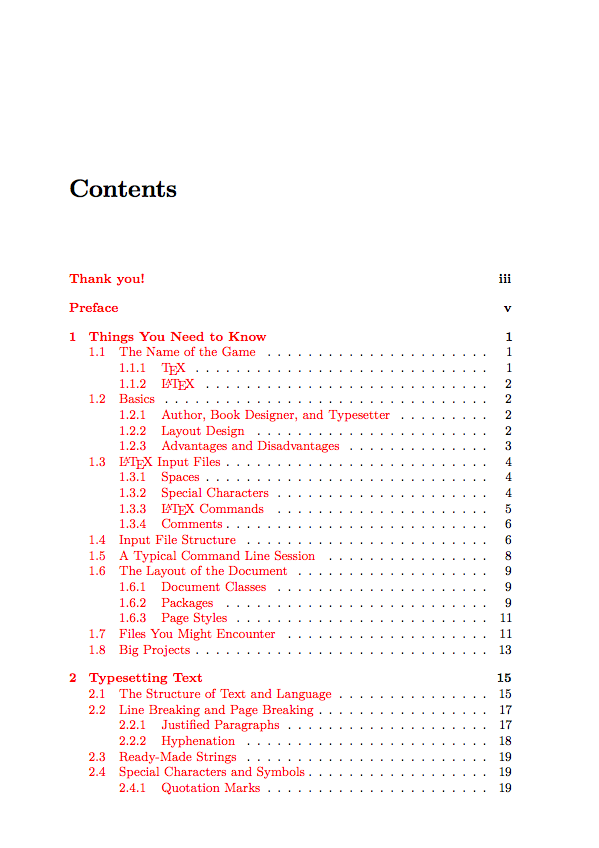
\includegraphics[width=5.1cm]{document1}
\end{figure}

\column{.5\textwidth}
\begin{figure}
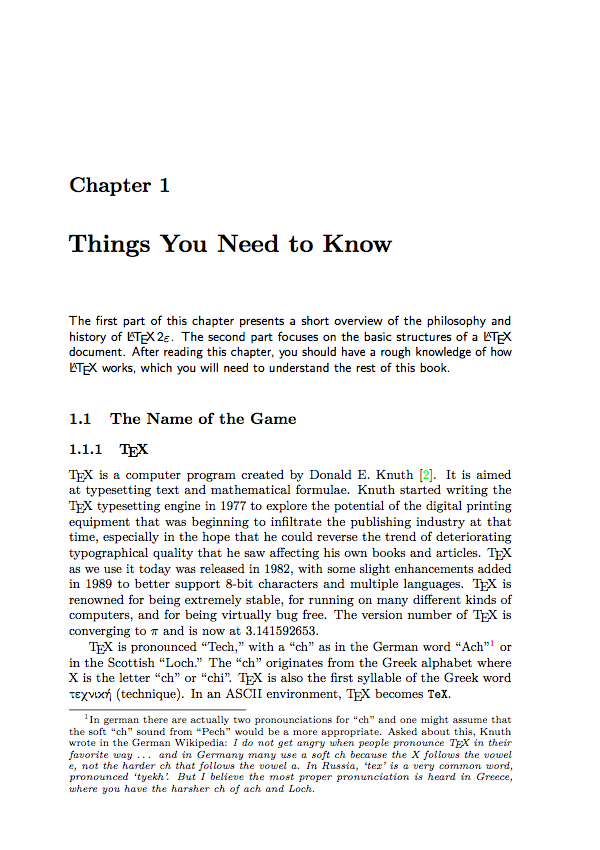
\includegraphics[width=5.1cm]{document2}
\end{figure}
\end{columns}

\end{frame}

%
\begin{frame}
\frametitle{Graceful Mathematical formulae}
\begin{tcolorbox}[colback=blue!5,colframe=blue!75!black] 
Add $a$ squared and $b$ squared to get $c$ squared. Or, using
a more mathematical approach:
\begin{displaymath}
c^{2}=a^{2}+b^{2}
\end{displaymath}
or you can type less with:
\[a+b=c\]
\end{tcolorbox}  

\end{frame}

%
\begin{frame}
\frametitle{Graceful Mathematical formulae}
\begin{tcolorbox}[colback=blue!5,colframe=blue!75!black] 
\newcommand{\ud}{\mathrm{d}}
\begin{displaymath}
\underbrace{a + \overbrace{b + \cdots + y}^{24} + z}_{26}
\end{displaymath}

\begin{displaymath}
y = \left\{ \begin{array}{ll}
 a & \textrm{if $d>c$}\\
 b+x & \textrm{in the morning}\\
 l & \textrm{all day long}
  \end{array} \right.
\end{displaymath}

\begin{displaymath}
E(u)=\int_{\Omega}\phi(|\nabla u|)+\lambda \int_{\Omega}(f-Ru)^2\ud x
\end{displaymath}  

\begin{displaymath}
p'(z)=c\sum_{k=1}^n \prod_{\substack{i=1 \\ i\neq k}}^n(z-r_i)=\sum_{k=1}^n p(z)/(z-r_k)
\end{displaymath} 
\end{tcolorbox}  

\end{frame}

%
\begin{frame}
\frametitle{Graceful Mathematical formulae}
\begin{tcolorbox}[colback=blue!5,colframe=blue!75!black]
\begin{displaymath}
\resizebox{1\hsize}{!}{$
\begin{bmatrix}
d_1 & c_1  &        &             &              &                 & \\
a_1 & d_2 & c_2 &             &              &                 & \\
      & a_2 & d_3 &   c_3    &              &                 & \\
      &        & a_3 &   d_4     & c_4      &                 &  \\
      &        &         & \ddots &\ddots  & \ddots    & \\
      &        &         &              &a_{n-2}&   d_{n-1} & c_{n-1}\\
      &        &         &              &               &   a_{n-1} & d_n
\end{bmatrix}
\begin{bmatrix}
x_1\\
x_2\\
x_3\\
x_4\\
\vdots\\
x_{n-1}\\
x_n
\end{bmatrix}
=\begin{bmatrix}
b_1\\
b_2\\
b_3\\
b_4\\
\vdots\\
b_{n-1}\\
b_n
\end{bmatrix}$}
\end{displaymath}
\end{tcolorbox} 
 
\end{frame}

%
\begin{frame}
\frametitle{Graceful Mathematical formulae}
\begin{tcolorbox}[colback=blue!5,colframe=blue!75!black]
\begin{eqnarray*}
(LU)_{ij}&=&\sum_{k=1}^{n}l_{ik}u_{kj}=\sum_{k=1}^{j}l_{ik}a_{kj}^{(k)}\\
&=&\sum_{k=1}^{j}(a_{ij}^{(k)}-a_{ij}^{(k+1)})\\
&=&a_{ij}^{(1)}-a_{ij}^{j+1}\\
&=&a_{ij}^{(1)}=a_{ij}
\end{eqnarray*}
\end{tcolorbox}
  
\end{frame}

%
\begin{frame}
\frametitle{Make a presentation}
\begin{itemize} 
\item Learn a few {\color{blue}easy-to-understand} commands that specify the logical structure of a document. 
\end{itemize}

\end{frame}

%
\begin{frame}[fragile]
\frametitle{Make a presentation}
\begin{lstlisting}[language={[LaTeX]TeX}]
\documentclass{beamer}
\usepackage[utf8]{inputenc}

%Information to be included in the title page:
\title{Sample title}
\author{Anonymous}
\date{2014}

\begin{document}

\begin{frame}
\frametitle{Sample frame title}
This is a text in first frame. 
\end{frame}  %

\end{document}
\end{lstlisting}

\end{frame}

%
\begin{frame}
\frametitle{Make a presentation}
\begin{figure}
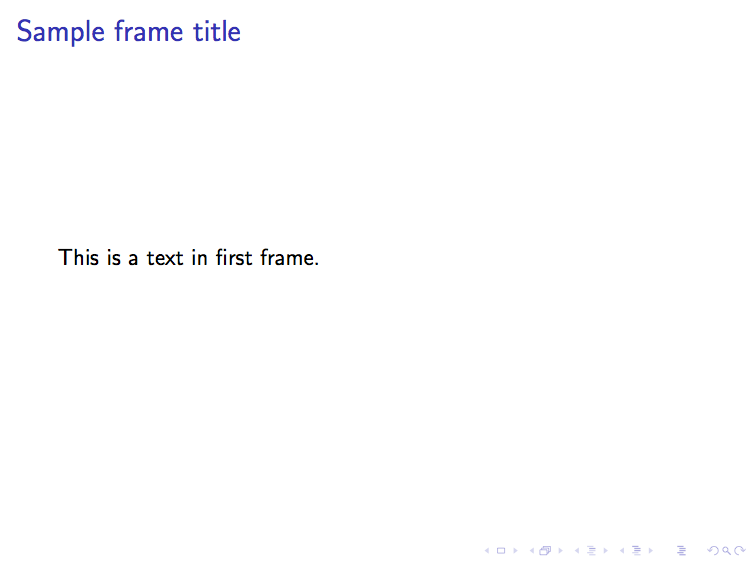
\includegraphics[width=10cm]{simplebeamer}
\end{figure}

\end{frame}


%
\begin{frame}
\frametitle{Free various packages }
%\begin{tcolorbox}[colback=blue!5,colframe=blue!75!black]
\begin{itemize}
\item Free add-on packages exist for many typographical tasks not directly supported by basic \LaTeX.
%\tcblower
\begin{itemize}
\begin{columns}
\begin{column}{\leftmargini}
\end{column}
\begin{column}{.5\linewidth}
\item {\color{red}C}{\color{orange}o}{\color{yellow}l}{\color{green}o}{\color{blue}u}{\color{gray}r}{\color{purple}e}{\color{red}d} {\color{violet}t}{\color{black}e}{\color{brown}x}{\color{red}t}
\item Include graphics.
\item Bring source code from a file into your document.
\item . . .
\end{column}
\begin{column}{0.5\linewidth}

\begin{figure}
 
\includegraphics[width=2cm]{cat}
\end{figure}

\end{column}
\end{columns}\vspace{1ex}
\end{itemize}
\end{itemize}
%\end{tcolorbox}  

\end{frame}

%
\begin{frame}
\frametitle{Multi-platform applications}
%\begin{tcolorbox}[colback=blue!5,colframe=blue!75!black] 
\begin{itemize}
\item \TeX, the formatting engine of \LaTeXe, is highly portable and free.
Therefore the system runs on almost any hardware platform available.
%\tcblower
\begin{center}
\begin{figure}

\includegraphics[width=5cm]{texcollection2014}
\end{figure}
\end{center}
\end{itemize}
%\end{tcolorbox}  

\end{frame}

%
\begin{frame}
\frametitle{$\cdots$ and more}
\begin{itemize}
\item Stable, Free and Open Source.
\item \LaTeX \;is very flexible, and will do the things you want.
\item $\cdots$
\end{itemize}

\end{frame}

\section{How does \LaTeX \;work?}

%
\begin{frame}
\frametitle{How does \LaTeX \;work?}
\begin{itemize}
\item<1> \LaTeX \;is a typesetting system
\begin{enumerate}
\item Taking a text file, containing \LaTeX \;commands, as input
\item Produces a PDF, DVI or PS file
\end{enumerate}
\item<2-> Create text file using editor and save as {\color{blue}some.tex}.
\item<2-> Compile the file using command
\begin{itemize}
\item use {\color{blue}latex some.tex} $\Rightarrow$ {\color{blue}some.dvi}
\item use {\color{blue}dvips some.dvi} $\Rightarrow$ {\color{blue}some.ps}
\item use {\color{blue}pdflatex(xelatex) some.tex} $\Rightarrow$ {\color{blue}some.pdf}
\end{itemize}
\end{itemize}

\end{frame}

\section{Some Interesting Applications}

%
\begin{frame}
\frametitle{Theorem}
\theoremstyle{plain}
\newtheorem{theorem}{THEOREM}
\begin{theorem}[Theorem on Matrix Inverse]
If $A$ and $B$ are square matrices such that $AB=I$, then $BA=I$.
\end{theorem}
\begin{proof}
Let $C=BA-I+B$. Then
\begin{equation*}
AC=ABA-AI+AB=A-A+I=I
\end{equation*}

Thus, $C$ (as well as $B$) is a right inverse of $A$. By Theorem 2, $B=C$; hence, $BA=I$.  
\end{proof}

\end{frame}

%
\begin{frame}
\frametitle{Table}
\begin{textblock*}{10cm}(4cm,3cm)
\begin{tabular}{|r|l|}
\hline
7C0 & hexadecimal \\
3700 & octal \\ \cline{2-2}
11111000000 & binary \\
\hline \hline
1984 & decimal \\
\hline
\end{tabular}
\end{textblock*}

\begin{textblock*}{10cm}(2cm,5.5cm)
\rowcolors[]{1}{blue!20}{blue!10}
\begin{tabular}{l!{\vrule}c|c|c|c}
Class & A & B & C & D \\
\hline
X & 1 & 2 & 3 & 4  \\
\hline
Y & 3 & 4 & 5 & 6  \\
\hline
Z & 5 & 6 & 7 & 8
\end{tabular}
\end{textblock*}

\begin{textblock*}{10cm}(6.5cm,5.5cm)
\begin{tabular}{|c|c|c|c|} 
\hline
资源限量&甲&乙&资源总数\\
\hline
煤&9&4&360\\
\hline
电&4&5&200\\
\hline
油&3&10&300\\
\hline
单位价格&7&12&*\\
\hline
\end{tabular}
\end{textblock*}

\end{frame}

%
\begin{frame}
\frametitle{Geometry}
\setlength{\unitlength}{0.8cm}
\begin{picture}(6,5)
\thicklines
\put(1,0.5){\line(2,1){3}}
\put(4,2){\line(-2,1){2}}
\put(2,3){\line(-2,-5){1}}
\put(0.7,0.3){$A$}
\put(4.05,1.9){$B$}
\put(1.7,2.95){$C$}
\put(3.1,2.5){$a$}
\put(1.2,1.7){$b$}
\put(2.5,1.05){$c$}
\put(0.3,4){$F=
\sqrt{s(s-a)(s-b)(s-c)}$}
\put(3.5,0.4){$\displaystyle
s:=\frac{a+b+c}{2}$}
\end{picture}

\end{frame}

%
\begin{frame}[fragile]
\frametitle{Insert Python scripts}
\begin{lstlisting}[language=Python]
#!/usr/local/bin/python
print "Hello World"
os.system("""
VAR=even;
sed -i "s/$VAR/odd/" testfile;
for i in `cat testfile` ;
do echo $i; done;
echo "now the tr command is removing the vowels";
cat testfile |tr 'aeiou' ' '
""") 
\end{lstlisting}

\end{frame}

%
\begin{frame}
\frametitle{Columns and Blocks}
\begin{block}{The OUC logo}
\begin{columns}
\begin{column}{.3\linewidth}

\includegraphics[height=3cm]{ouc-logo.png}
\end{column}
\begin{column}{.6\linewidth}
This is the logo of OUC.\\
海纳百川,取则行远。
\end{column}
\end{columns}
\end{block}

\end{frame}

%
\begin{frame}
\frametitle{Figures}
\shadow{生物形态学分类特征}
形状、突起、角毛
\begin{figure}
\begin{minipage}[t]{0.25\linewidth} 
\centering 
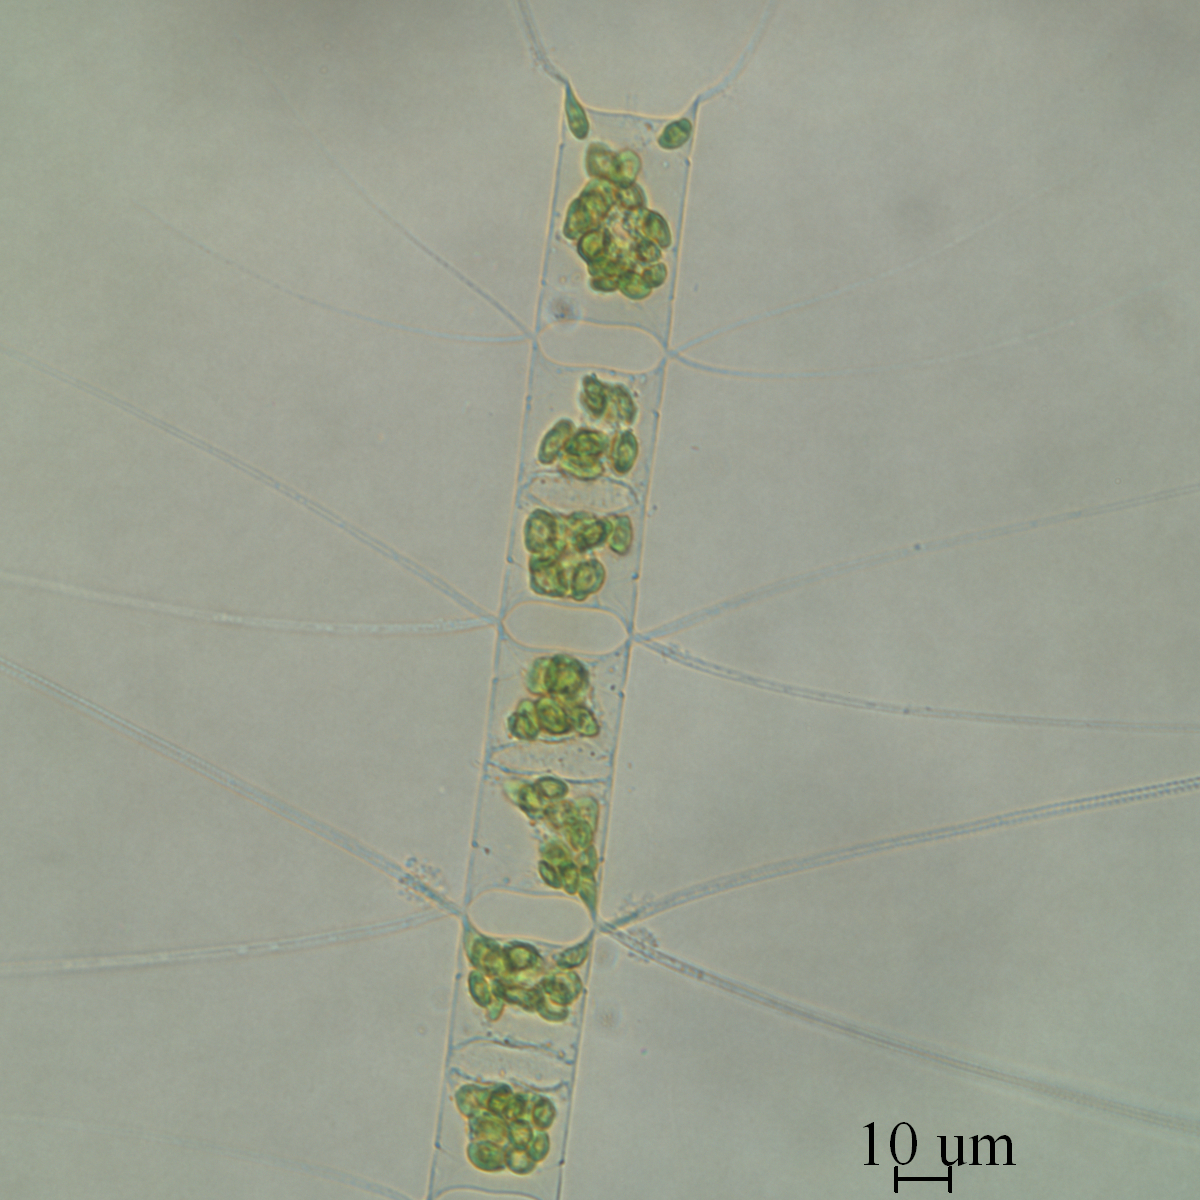
\includegraphics[width=\linewidth]{20081112-LuoShiJiaoMaoZao.png} \\
    洛氏角毛藻
\end{minipage} 
\begin{minipage}[t]{0.25\linewidth} 
\centering 
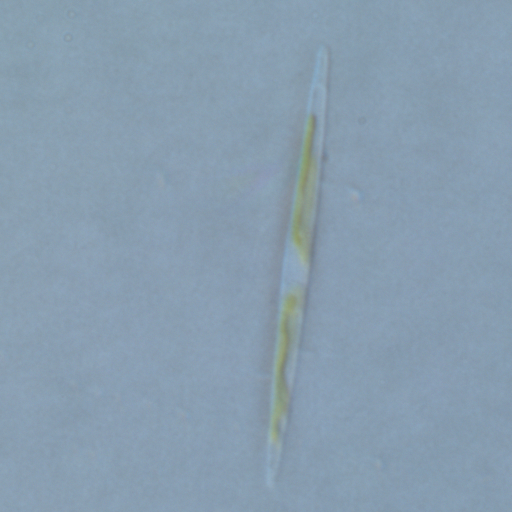
\includegraphics[width=\linewidth]{20080512-JianCiNiLingXingZao.png}\\ 
    {\heiti\textcolor{red}{尖刺伪菱形藻}}
\end{minipage} 
\\
\begin{minipage}[t]{0.25\linewidth} 
\centering 
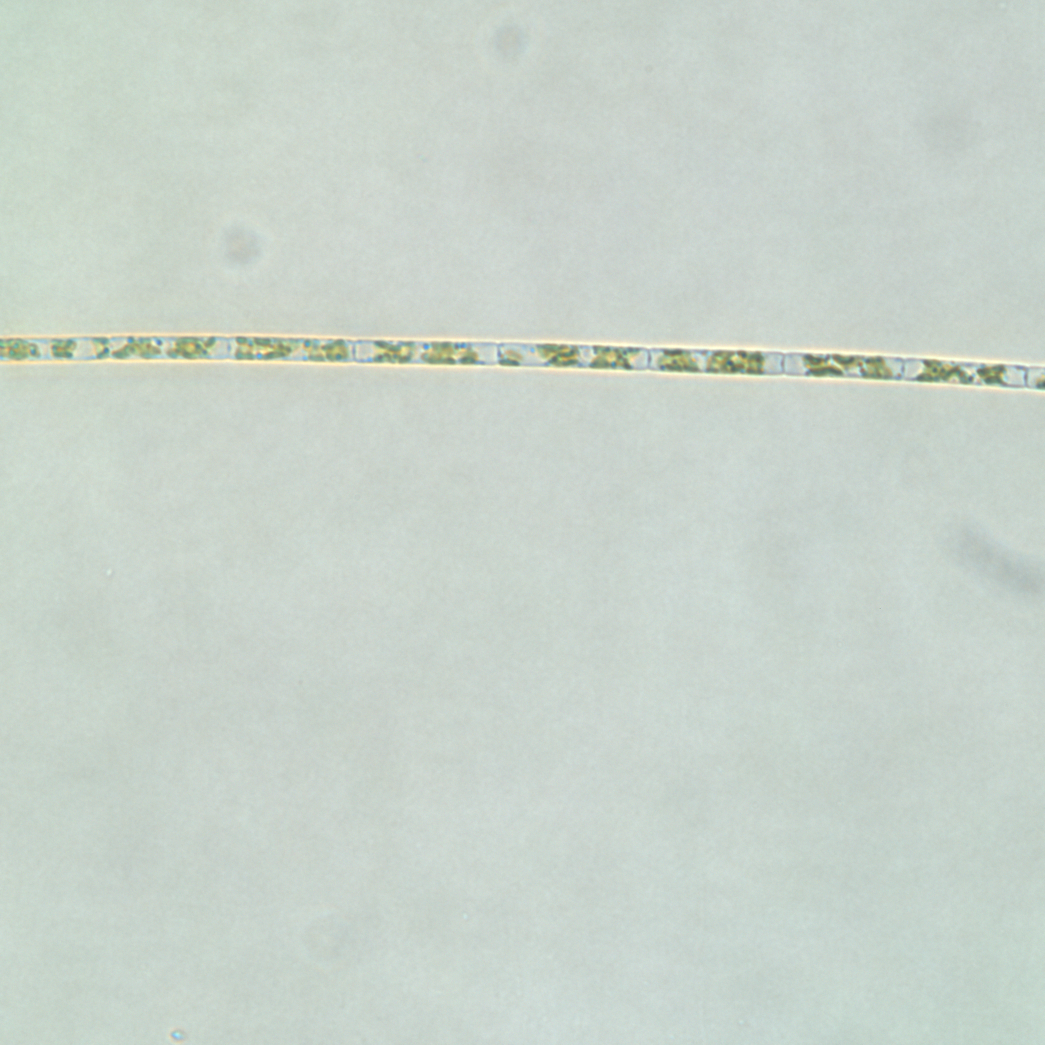
\includegraphics[width=\linewidth]{20081112-DanMaiXiZhuZao.png}\\ 
    丹麦细柱藻
\end{minipage} 
\begin{minipage}[t]{0.25\linewidth} 
\centering 
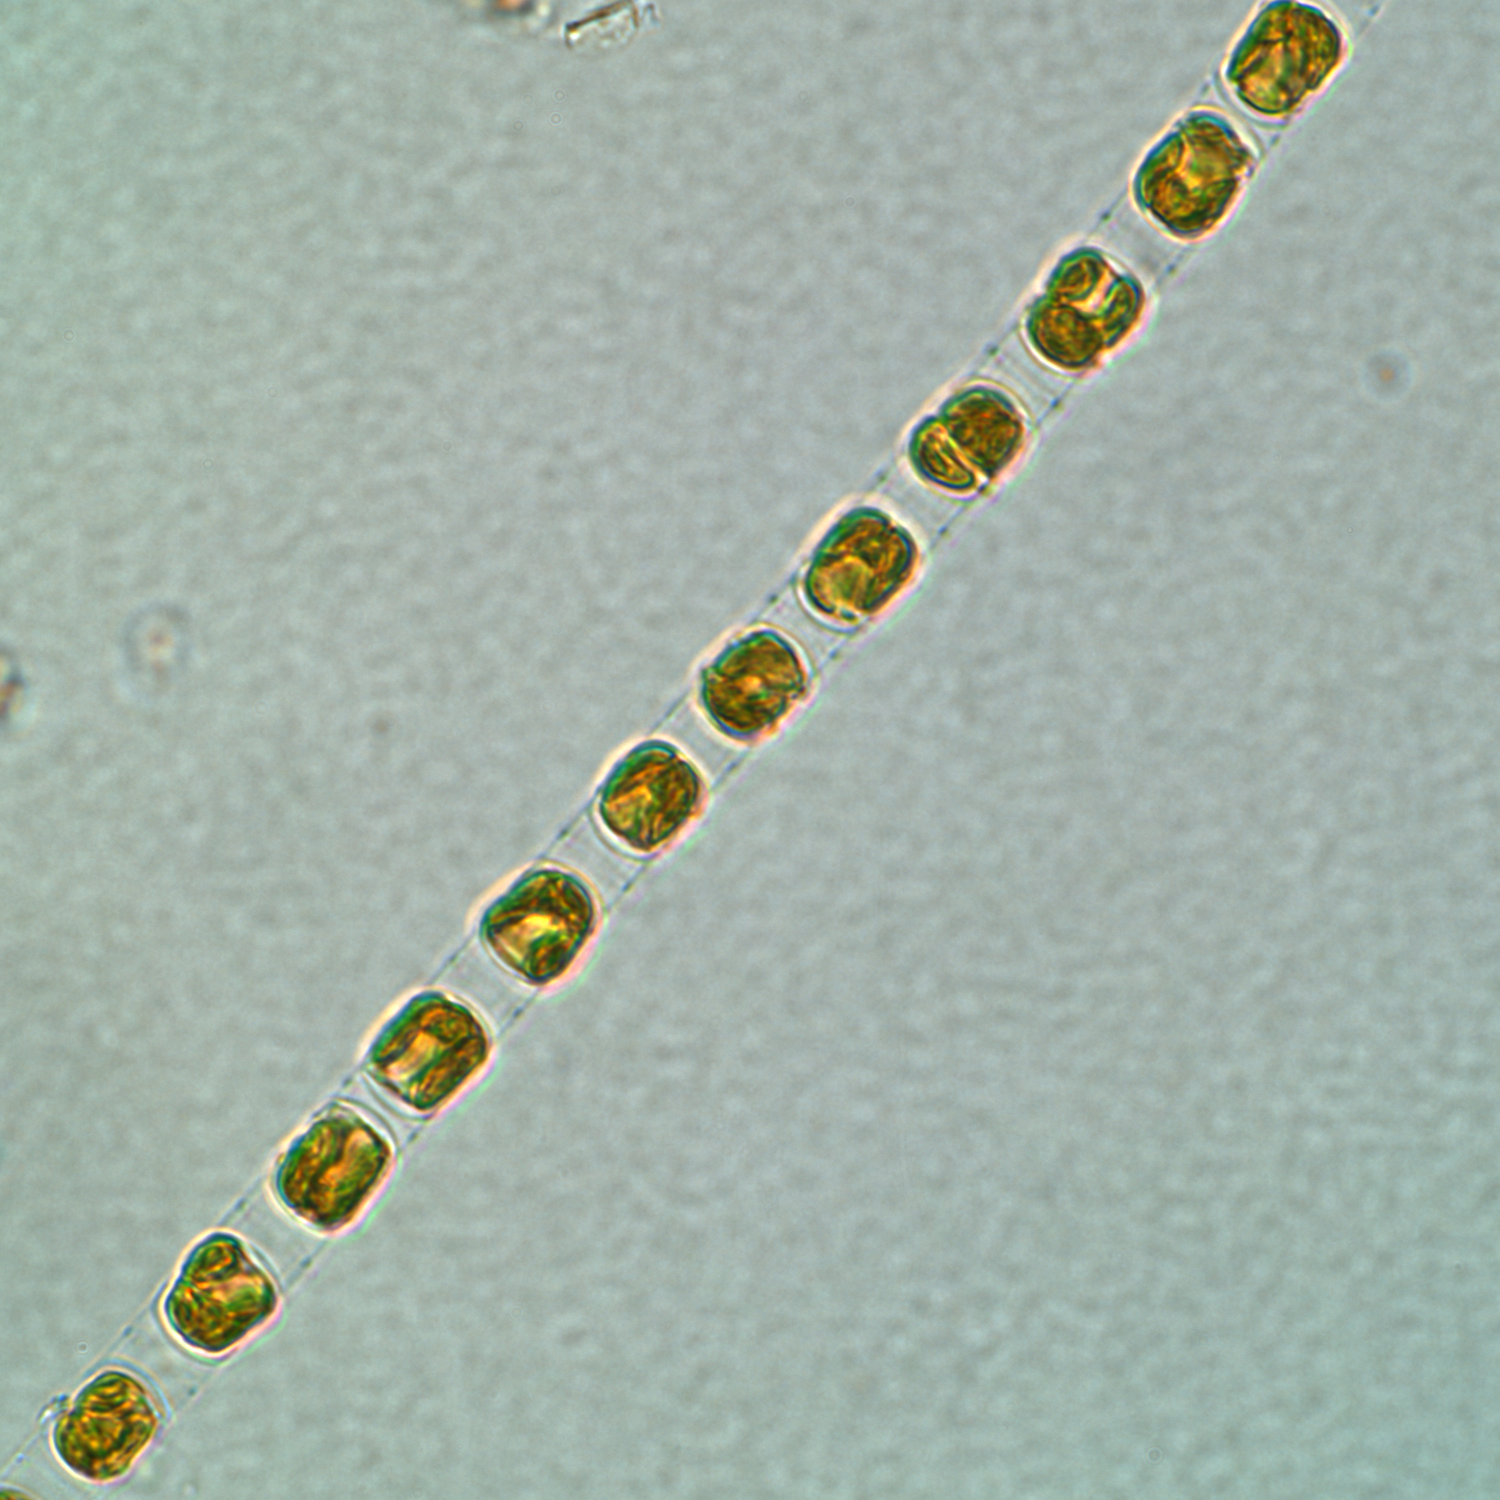
\includegraphics[width=\linewidth]{20081112-ReDaiGuTiaoZao.png}\\
    {\heiti\textcolor{red}{热带骨条藻}}
\end{minipage} 
\end{figure}

\end{frame}

%
\begin{frame}
\frametitle{Some Interesting Applications}
{\scriptsize
\begin{center}
\resizebox{1\hsize}{!}{$
\begin{tabular}{rl}
{\normalsize\hei 硅藻门~\textbf{3/12}}
&\rowcolors[]{1}{blue!18}{blue!7}
\begin{tabular}[!ht]{cccc}
  22 & 旋链角毛藻 & \emph{Chaetoceros curvisetus} & \\
  23 & 洛氏角毛藻 & \emph{Chaetoceros lorenzianus} & $\surd$ \\
  24 & 聚生角毛藻 & \emph{Chaetoceros socialis} & \\
  \textbf{\textcolor{red}{25}} & {\hei\textcolor{red}{尖刺伪菱形藻}} & \textbf{\emph{\textcolor{red}{Pseudo-nitzschia pungens}}} & ${\textcolor{red}{\surd}}$ \\
  \textbf{\textcolor{red}{26}} & {\hei\textcolor{red}{多纹伪菱形藻}} & \textbf{\emph{\textcolor{red}{Pseudo-nitzschia multistriata}}} & \\
  27 & 丹麦细柱藻 & \emph{Leptocylindrus danicus} & $\surd$ \\
  28 & 新月筒柱藻 & \emph{Cylindrotheca closterium} & \\
  29 & 派格棍形藻 & \emph{Bacilaria paxillifera} & \\
  \textbf{\textcolor{red}{30}} & {\hei\textcolor{red}{热带骨条藻}} & \textbf{\emph{\textcolor{red}{Skeletonema tropicum}}} & ${\textcolor{red}{\surd}}$ \\
  31 & 旋转海链藻 & \emph{Thalassiosira curviseriata} & \\
  32 & 圆海链藻 & \emph{Thalassiosira rotula} & \\
  33 & 双环海链藻 & \emph{Thalassiosira diporocyclus} & \\
\end{tabular}
\\
&
\\
{\normalsize\hei 针胞藻纲~\textbf{2/2}}
&\rowcolors[]{1}{blue!18}{blue!7}
\begin{tabular}[!ht]{cccc}
  \textbf{\textcolor{red}{34}} & \hspace{0.6em}{\hei\textcolor{red}{海洋卡盾藻}}\hspace{0.09cm} & \hspace{1em}\hspace{0.68cm}\textbf{\emph{\textcolor{red}{Chattonella marina}}}\hspace{0.54cm} & ${\textcolor{red}{\surd}}$ \\
 \textbf{\textcolor{red}{35}} & \hspace{0.6em}{\hei\textcolor{red}{赤潮异湾藻}}\hspace{0.09cm} & \hspace{1em}\textbf{\emph{\textcolor{red}{Heterosigma akashiwo}}} & ${\textcolor{red}{\surd}}$ \\
\end{tabular}
\\
&
\\
{\normalsize\hei 硅鞭藻纲~\textbf{0/2}}
&\rowcolors[]{1}{blue!18}{blue!7}
\begin{tabular}[!ht]{cccc}
  \hspace{0.01cm}36\hspace{0.01cm} & 小等刺硅鞭藻\hspace{0.007cm} & \hspace{1.09cm}\emph{Dictyochafibula}\hspace{1.2cm} & $\surd$ \\
  37 & 六异刺硅鞭藻\hspace{0.007cm} & \emph{Distephanus speculum} & \\
\end{tabular}
\\
&
\\
{\normalsize\hei 隐藻门~\textbf{0/1}}
&\rowcolors[]{1}{blue!18}{blue!7}
\begin{tabular}[!ht]{cccc}
  \hspace{0.01cm}38\hspace{0.01cm} & \hspace{0.25cm}抢鞋隐藻\hspace{0.28cm} & \hspace{0.41cm}\emph{Cryptomonas calceiformis}\hspace{0.41cm} & \hspace{1.3em} \\
\end{tabular}
\\
{\normalsize\hei 定鞭藻纲~\textbf{1/1}}
&\rowcolors[]{1}{blue!18}{blue!7}
\begin{tabular}[!ht]{cccc}
  \textbf{\textcolor{red}{39}} & \hskip0.5em{\hei\textcolor{red}{球形棕囊藻}}\hspace{0.09cm} & \hspace{0.73cm}\textbf{\emph{\textcolor{red}{Phaeocystis globosa}}}\hspace{0.73cm} & $\textcolor{red}{\surd}$ \\
\end{tabular}
\\
{\normalsize\hei 蓝藻门~\textbf{0/1}}
&\rowcolors[]{1}{blue!18}{blue!7}
\begin{tabular}[!ht]{cccc}
  \hspace{0.01cm}40\hspace{0.01cm} & \hskip0.6em 红海束毛藻\hspace{0.09cm} & \hspace{0.34cm}\emph{Trichodesminu erythraeum}\hspace{0.41cm} & $\surd$ \\
\end{tabular}
\\
\end{tabular}$}
\end{center}
}
\end{frame}

%
\begin{frame}
\frametitle{Circuit diagram}
\begin{center}
\begin{tikzpicture}[scale=0.7]
\draw [->] (0,0) node [left] {$O$} -- (6,0) node [right] {$f$};
\draw [->] (0,0) -- (0,3) node [left] {$A_{u}$};
\draw [dashed] (0,1.414) node [left] {$0.707A_{um}$} -- (5.8,1.414);
\draw [dashed] (0,2) node [left] {$A_{um}$} -- (5.8,2);
\draw [thick] (0.5,0.5) parabola [bend at end] (1.5,2) -- (4.5,2) parabola [bend at start] (5.5,0.5);
\draw [dashed] (0.9,0) -- (0.9,1.414);
\draw [dashed] (5.1,0) -- (5.1,1.414);
\draw [<->] (0.9,0.7) -- node [midway,auto] {$2\Delta f_{0.7}$} (5.1,0.7);
\end{tikzpicture}
\hspace{-1cm}
\begin{tikzpicture}[>=stealth']
\draw [->] (0,0) node [below] {$0$} -- (3.5,0) node [below] {$f$};
\draw [->] (0,0) -- (0,4) node [left] {$K$};
\draw [thick] (1,0.2) parabola bend (2,3.5) (3,0.2);
\draw [dashed] (2,3.5) -- (2,0) node [below] {$f_0$};
\draw [dashed] (2,3.5) -- (0,3.5) node [left] {$K_0$};
\draw [dashed] (0,2.45) node [left] {$0.7K_0$} -- (2.6,2.45);
\draw [->] (0.5,2.45) -- node [midway,auto] {$\Delta f_{0.7}$} (1.45,2.45);
\draw [->] (3.5,2.45) -- node [midway,auto,swap] {$\Delta f_{0.7}$} (2.55,2.45);
\draw [dashed] (1.45,2.45) -- (1.45,4);
\draw [dashed] (2.55,2.45) -- (2.55,4);
\draw [<->] (1.45,3.8) -- node [midway,auto] {$2\Delta f_{0.7}$} (2.55,3.8);
\draw [dashed] (0,1) node [left] {$K$} -- (2.9,1);
\draw [dashed] (2.85,1) -- (2.85,0) node [below] {$f_1$};
\draw [<->] (2,0.3) -- node [midway,auto] {$\Delta f$} (2.85,0.3);
\end{tikzpicture}      
\end{center}
\end{frame}

%
\begin{frame}
\frametitle{CV or resume }
\begin{figure}
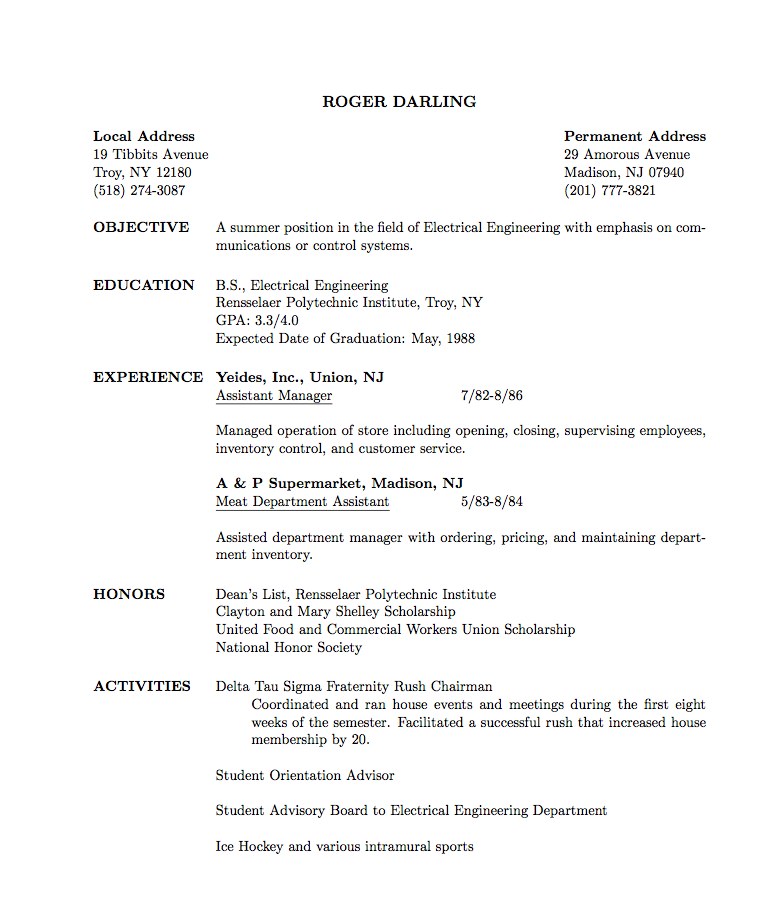
\includegraphics[width=6.5cm]{cv}
\end{figure}

\end{frame}


\section{\LaTeX \;and Research}

%
\begin{frame}
\frametitle{Specialities}
\begin{itemize}
\item\LaTeX \;is proper to create, edit and publish your research.\begin{itemize}
\item Thesis
\item Conference papers
\item Journal papers
\item Book
\item $\cdots$
\end{itemize}
\end{itemize}

\end{frame}

%
\begin{frame}
\frametitle{\LaTeX\;and zhenglab}
\begin{figure}
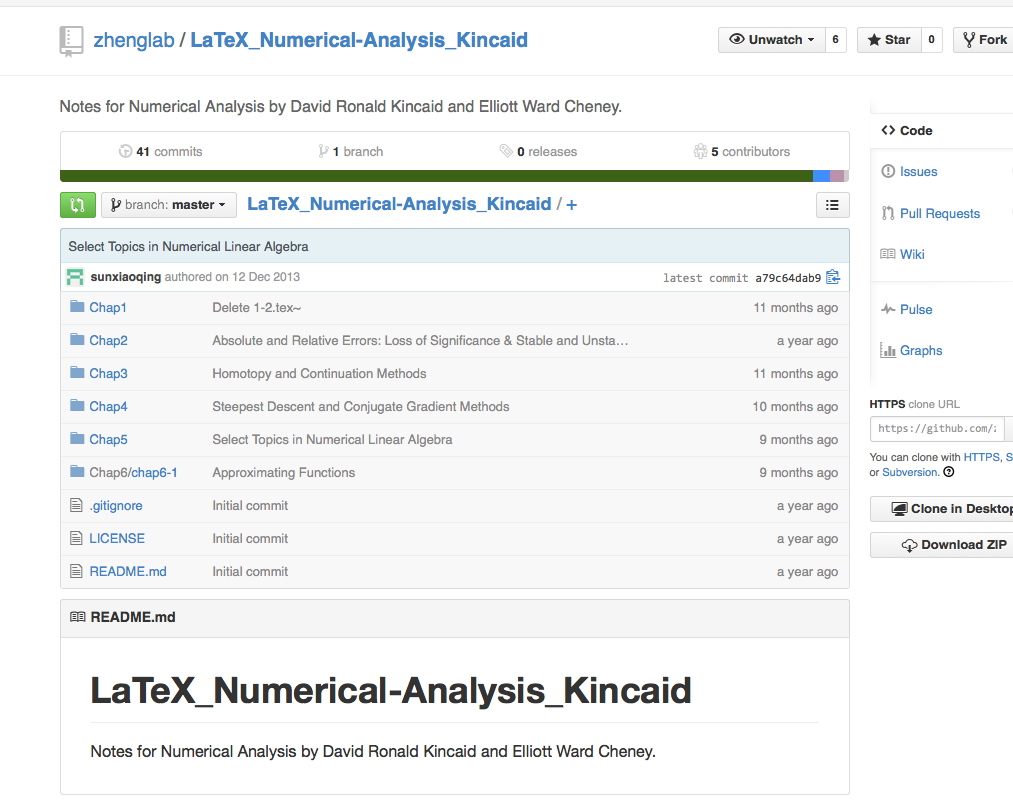
\includegraphics[width=9cm]{github}
\end{figure}
\end{frame}

%
\begin{frame}[fragile]
\frametitle{\LaTeX\;and zhenglab}
\begin{columns}[c]
\column{0.5\textwidth}
\begin{figure}
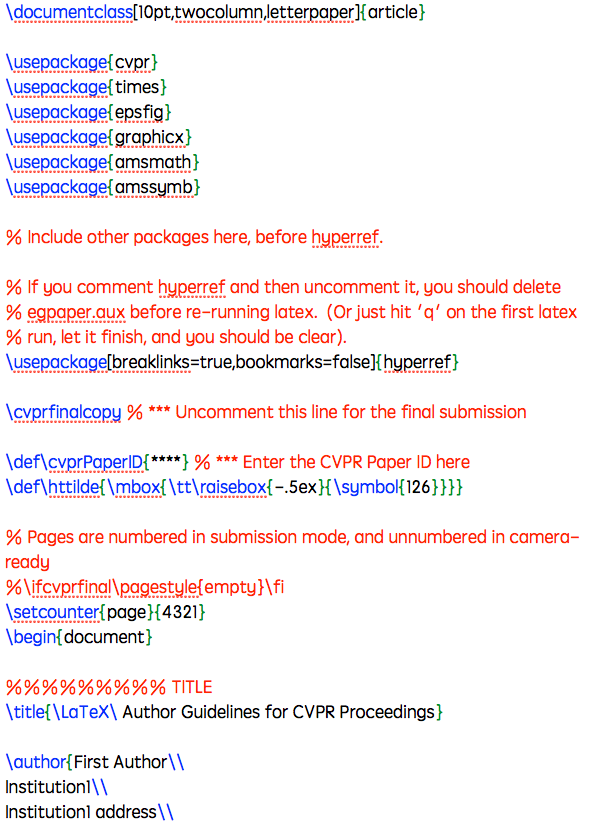
\includegraphics[width=5.1cm]{cvpr1}
\end{figure}

\column{0.5\textwidth}
\begin{figure}
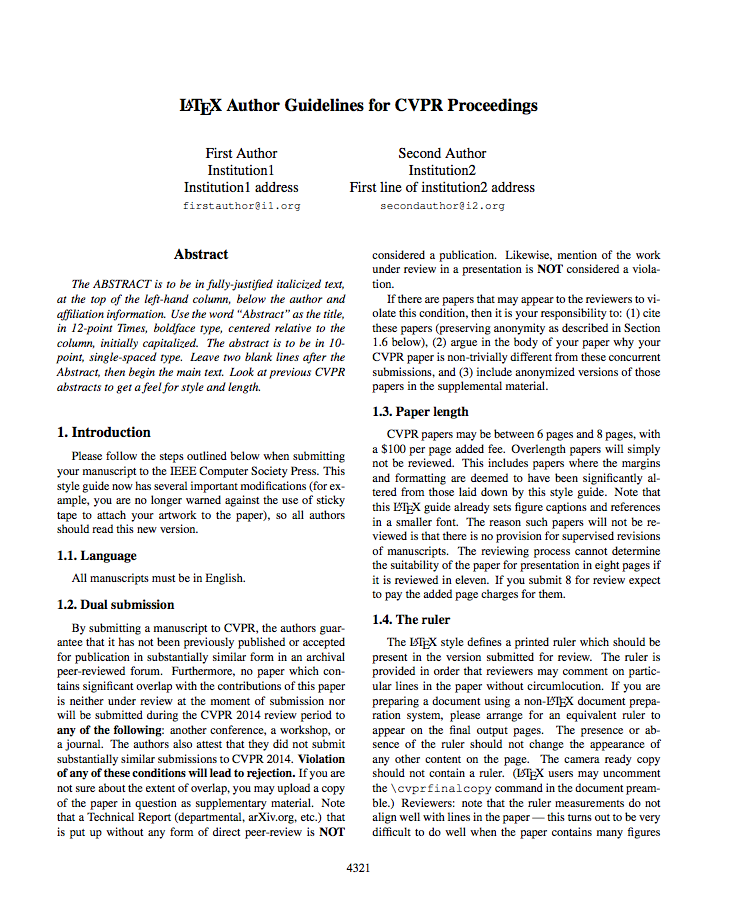
\includegraphics[width=5.2cm]{cvpr2}
\end{figure}
\end{columns}

\end{frame}

%
\begin{frame}
\frametitle{Some Resources} 
\begin{itemize}
\item TeX Users Group web site: \url{http://www.tug.org/}
\item More usepackages can be found: \url{http://www.ctan.org/}
\item \LaTeX\;help document: \small{\url{http://www.ctan.org/tex-archive/info/lshort}}
\item \normalsize{BibTeX web site: \url{http://www.bibtex.org/}}
\item BibDesk web site: \url{http://bibdesk.sourceforge.net/}
\end{itemize}

\end{frame}

%
\begin{frame}
\begin{figure}\centering
\begin{minipage}[t]{0.7\linewidth}

\includegraphics[width=\linewidth]{thank.jpg}
\end{minipage}
\end{figure}

\end{frame}


\end{document}